\documentclass{article}

\usepackage[utf8]{inputenc}
\usepackage[english]{babel}
\usepackage[parfill]{parskip}
\usepackage{graphicx}

\begin{document}

  \newcommand{\version}[0]{1.1-SNAPSHOT}
  \newcommand{\KiekerTraceDiagnosis}[0]{\texttt{Kieker Trace Diagnosis}}
  \newcommand{\file}[1]{\textit{#1}}

  \title{Kieker Trace Diagnosis\\Benutzerhandbuch}
  \date{Version \version{}}
  \author{Kieker Project\\(kieker-monitoring.net)}

  \maketitle

  \section{Anforderungen und Installation}
  Die folgenden Anforderungen sind notwendig, um \KiekerTraceDiagnosis{} verwenden zu können.
  \begin{itemize}
    \item Windows oder Linux
    \item Java Runtime Environment 8
  \end{itemize}
  Für die Verwendung des Werkzeuges wird das Oracle JDK empfohlen. Die Problembehandlung bei Verwendung des OpenJDK findet sich in Abschnitt~\ref{OpenJDK}.\\

  Zur Installation muss lediglich das Archiv \file{Kieker Trace Diagnosis-\version{}-linux.tgz}, beziehungsweise \file{Kieker Trace Diagnosis-\version{}-windows.zip}, in einen beliebigen Ordner entpackt werden.
  Die Anwendung kann anschließend über das Startscript \file{start.sh}, beziehungsweise \file{start.bat}, im Ordner \file{bin} gestartet werden.
  Die Anwendung sollte in dem Verzeichnis, aus welchem das Startscript heraus aufgerufen wird, Schreibrechte besitzen.

  \section{Ansichten}

  \subsection{Einstellungen}

  Das Fenster \textit{Einstellungen} ermöglicht die Konfiguration des Werkzeuges.

  \begin{figure}[h]
    \centering
    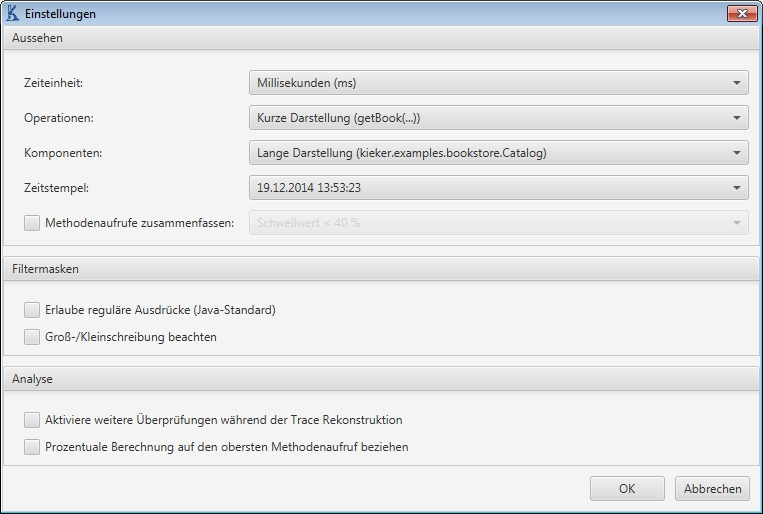
\includegraphics[width=0.8\textwidth]{img_DE/Einstellungen.jpg}
  \end{figure}

  \paragraph{Zeiteinheit}
  Hier kann eingestellt werden, in welcher Zeiteinheit die Dauer von Methodenaufrufen und ähnlichem angezeigt werden.
  Dies ist beispielsweise dann sinnvoll, wenn Daten mit Auflösung im Nanosekunden-Bereich gesammelt wurden, die interessanten Methodenaufrufe sich aber eher im Bereich von einigen Millisekunden befinden.

  \paragraph{Operationen}
  Hier kann eingestellt werden, in welcher Form Operationen dargestellt werden.
  Zur Auswahl sind eine verkürzte und eine ausführliche Darstellung.

  \paragraph{Komponenten}
  Hier kann eingestellt werden, in welcher Form Komponenten dargestellt werden.
  Zur Auswahl sind eine verkürzte und eine ausführliche Darstellung.

  \paragraph{Zeitstempel}
  Hier kann eingestellt werden, in welcher Form Zeitstempel von Methodenaufrufen und ähnlichem angezeigt werden.
  Zur Auswahl sind diverse Zeit- und Datumsformate.

  \paragraph{Methodenaufrufe zusammenfassen}
  Hier kann eingestellt werden, ob unsignifikante Methodenaufrufe in Traces zusammengefasst werden sollen.
  Das is beispielsweise dann sinnvoll, wenn Traces mit einigen tausend Methodenaufrufen betrachtet werden, von denen die meisten sehr schnell abgearbeitet wurden und uninteressant sind.  
  Methoden unterhalb des gegebenen Schwellwertes werden zusammengefasst, sodass nur die signifikanteren und länger andauernden Methoden noch sichtbar sind.

  \paragraph{Erlaube reguläre Ausdrücke (Java-Standard)}
  Mit dieser Einstellungen können in den Filtermasken reguläre Ausdrücke nach Java-Standard eingegeben werden.
  Wenn diese Option deaktiviert ist, findet eine Volltextsuche des eingegebenen Textes für das jeweilige Element statt.

  \paragraph{Groß-/Kleinschreibung beachten}
  Hier kann eingestellt werden, ob Groß- und Kleinschreibung in den Filtermasken beachtet wird oder nicht.

  \paragraph{Aktiviere weitere Überprüfungen während der Trace Rekonstruktion}

  \paragraph{Prozentuale Berechnung auf den obersten Methodenaufruf beziehen}

  \subsection{Traces}
  \subsection{Aggregierte Traces}
  \subsection{Methodenaufrufe}
  \subsection{Aggregierte Methodenaufrufe}
  \subsection{Monitoring Log Statistiken}

  \section{Lizenz}
  \KiekerTraceDiagnosis{} ist unter der Apache License Version 2.0 lizenziert. Der vollständige Lizenztext lässt sich der mitgelieferten Datei \file{LICENSE} entnehmen.

  \section{Fehlerbehebung}

  \subsection{Verwendung von OpenJDK}\label{OpenJDK}
  Die Verwendung von OpenJDK anstelle des Oracle JDKs ist grundsätzlich möglich. Es kann allerdings notwendig sein, OpenJFX explizit zu installieren.

  \subsection{Unable to create file logs/Kieker Trace Diagnosis.log}\label{LogSchreibrechte}
  Kommt es beim Start zu dieser Fehlermeldung, so hat \KiekerTraceDiagnosis{} vermutlich in dem aktuellen Arbeitsverzeichnis keine Schreibrechte.
  Die Anwendung kann dann keine Log-Dateien schreiben, kann aber wie gehabt verwendet werden.

\end{document}